\begin{figure}[htbp]
  \centering 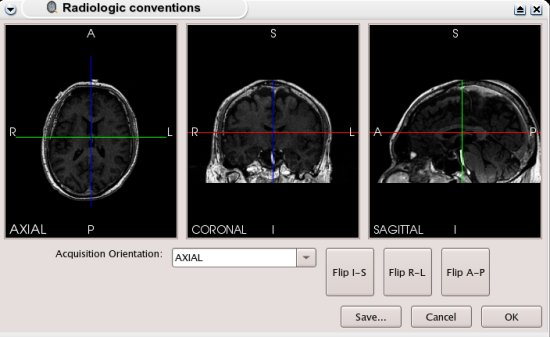
\includegraphics[width=0.75\linewidth]{reorientationtool}
  \caption{{\bf The Reorientation Tool main window. }
  \label{fig:reorientationtool}}
\end{figure}

This tool helps the user to manually re-orientate the image if this one doesn't match the
radiologic conventions correctly. The 3 views correspond respectively to the axial view,
the coronal view and the sagittal view of the image. 
\ \\

If the image has been acquired in another direction than axial, you can switch the
acquisition orientation flag in the check box. If the image is still flipped over an axis,
you can use switch the flipping flags for the three directions. I-S corresponds to
Inferior-Superior direction, R-L to Right-Left, and A-P to Anterior-Posterior. 
\ \\

Once the image meets correctly the conventions, you may want to save it in this
orientation by clicking ``save''. The image will be saved in ITK analyze format (.hdr -
.img) if no extension is given.
\ \\
